% ============================================================
% Of Two Minds at the Penalty Spot: Why Indecision Has a
% Neural Cost in the Goalkeeper–Striker Duel
% ============================================================
\documentclass[11pt,twocolumn]{article}

% --- Packages ---
\usepackage[utf8]{inputenc}
\usepackage[T1]{fontenc}
\usepackage{amsmath,amssymb}
\usepackage{graphicx}
\usepackage[margin=2cm]{geometry}
\usepackage{natbib}
\usepackage{hyperref}
\usepackage{xcolor}
\usepackage{booktabs}
\usepackage{caption}
\usepackage{float}

% --- Auto-generated statistics from analysis pipeline ---
% ============================================================
% AUTO-GENERATED — do not edit by hand.
% Regenerated every time `make` or `run_all.py` is executed.
% ============================================================
\newcommand{\PredOneNTotal}{482}
\newcommand{\PredOneNWithin}{225}
\newcommand{\PredOneNCross}{62}
\newcommand{\PredOneNMatch}{195}
\newcommand{\PredOneConvWithin}{95.6\%}
\newcommand{\PredOneConvCross}{95.2\%}
\newcommand{\PredOneConvMatch}{65.1\%}
\newcommand{\PredOneFisherOR}{1.09}
\newcommand{\PredOneFisherP}{0.5598}
\newcommand{\PredOneChiSq}{76.46}
\newcommand{\PredOneChiP}{0.0000}
\newcommand{\PredTwoNMultiMatches}{568}
\newcommand{\PredTwoNPairs}{622}
\newcommand{\PredTwoGoalAfterGoal}{77.4\%}
\newcommand{\PredTwoGoalAfterSave}{65.3\%}
\newcommand{\PredTwoNAfterGoal}{478}
\newcommand{\PredTwoNAfterSave}{144}
\newcommand{\PredTwoChiSq}{7.96}
\newcommand{\PredTwoChiP}{0.0048}
\newcommand{\PredTwoKaggleNSameMatch}{16}
\newcommand{\PredTwoKaggleRepeatRate}{75.0\%}
\newcommand{\PredTwoKaggleBinomP}{0.0008}
\newcommand{\PredFourNTotal}{4599}
\newcommand{\PredFourOverallSave}{18.6\%}
\newcommand{\PredFourLinCoef}{-0.0058}
\newcommand{\PredFourLinP}{0.5214}
\newcommand{\PredFourQuadCoef}{-0.00233}
\newcommand{\PredFourQuadP}{0.2211}
\newcommand{\PredFourLRChi}{1.52}
\newcommand{\PredFourLRP}{0.2170}
\newcommand{\PredFourPeakExp}{5.6}
\newcommand{\PredFourAICLin}{4423.8}
\newcommand{\PredFourAICQuad}{4424.2}
\newcommand{\PredFourSpearmanRho}{-0.386}
\newcommand{\PredFourSpearmanP}{0.0932}
\newcommand{\PredFiveNCentral}{12}
\newcommand{\PredFiveNDive}{470}
\newcommand{\PredFiveConvCentral}{83.3\%}
\newcommand{\PredFiveConvDive}{83.2\%}
\newcommand{\PredFiveFisherOR}{1.01}
\newcommand{\PredFiveFisherP}{0.6267}
\newcommand{\PredFiveZStat}{0.01}
\newcommand{\PredFiveZP}{0.5052}
\newcommand{\PredSixNNatural}{247}
\newcommand{\PredSixNUnnatural}{181}
\newcommand{\PredSixNCentre}{54}
\newcommand{\PredSixConvNatural}{81.4\%}
\newcommand{\PredSixConvUnnatural}{83.4\%}
\newcommand{\PredSixConvCentre}{90.7\%}
\newcommand{\PredSixFisherOR}{0.87}
\newcommand{\PredSixFisherP}{0.7496}
\newcommand{\PredSixLogitNatCoef}{0.182}
\newcommand{\PredSixLogitNatP}{0.5227}
\newcommand{\PredSixLogitMatchCoef}{-2.487}
\newcommand{\PredSixLogitMatchP}{0.0000}


% --- Colors ---
\definecolor{keeperblue}{HTML}{3B82F6}
\definecolor{strikerred}{HTML}{EF4444}
\definecolor{fieldgreen}{HTML}{10B981}
\definecolor{warncolor}{HTML}{F59E0B}
\definecolor{muted}{HTML}{6B7280}
\definecolor{boxbg}{HTML}{F0F9FF}
\definecolor{boxbg2}{HTML}{FFF7ED}

% --- Hyperref Setup ---
\hypersetup{
    colorlinks=true,
    linkcolor=keeperblue,
    citecolor=fieldgreen,
    urlcolor=keeperblue
}

% --- Custom Commands ---
\newcommand{\task}[1]{\textbf{#1}}
\newcommand{\region}[1]{\textsc{#1}}

% --- Tip Box Environments (using fbox) ---
\newenvironment{keeperbox}{%
  \smallskip\noindent\fcolorbox{keeperblue}{boxbg}{\begin{minipage}{\dimexpr\columnwidth-2\fboxsep-2\fboxrule}%
  {\small\sffamily\textcolor{keeperblue}{\textbf{Goalkeeper's Edge}}}\\[2pt]\small}%
  {\end{minipage}}\smallskip}

\newenvironment{strikerbox}{%
  \smallskip\noindent\fcolorbox{strikerred}{boxbg2}{\begin{minipage}{\dimexpr\columnwidth-2\fboxsep-2\fboxrule}%
  {\small\sffamily\textcolor{strikerred}{\textbf{Striker's Edge}}}\\[2pt]\small}%
  {\end{minipage}}\smallskip}

\newenvironment{caveatbox}{%
  \smallskip\noindent\fcolorbox{muted}{white}{\begin{minipage}{\dimexpr\columnwidth-2\fboxsep-2\fboxrule}%
  {\small\sffamily\textbf{Caveat Emptor}}\\[2pt]\small\itshape}%
  {\end{minipage}}\smallskip}

% ============================================================
\title{\textbf{Of Two Minds at the Penalty Spot}\\[0.3em]
\large Why Indecision Has a Neural Cost in the\\
Goalkeeper--Striker Duel}

\author{Kyle E. Mathewson\\
\small Department of Psychology, University of Alberta\\
\small Edmonton, Alberta, Canada\\
\small \texttt{kyle.mathewson@ualberta.ca}}

\date{\small Draft --- \today}

% ============================================================
\begin{document}
\maketitle

% ============================================================
\begin{abstract}
Coaches tell penalty takers to ``pick a side and commit''---don't be \emph{of two minds}.
But why, exactly, does indecision hurt?
The penalty kick is among the most dramatic moments in sport: a goalkeeper and striker locked in a rapid duel of anticipation, deception, and motor commitment.
Existing accounts frame this contest through game theory \citep{palacioshuerta2003minimax}, action bias \citep{bareli2007action}, or perceptual expertise \citep{mann2007perceptual}.
Here, I propose a complementary neuroscience-grounded framework drawn from recent evidence that the primate brain performs multiple tasks by compositionally engaging shared neural subspaces \citep{tafazoli2026compositional}.
I argue that being ``of two minds''---maintaining two competing action plans simultaneously---has a specific neural cost: both goalkeeper and striker execute their decisions by combining sensory categorisation and motor response subspaces that are \emph{shared} across different action plans.
This sharing confers efficiency---enabling flexible, compositional behaviour---but also creates predictable interference when two potential actions occupy the same motor axis.
I derive seven testable predictions and evaluate five of them against two public penalty kick datasets ($N = \PredOneNTotal$ penalties from multiple national leagues and $N = \PredFourNTotal$ Bundesliga penalties from 1963--2017).
The most striking result concerns sequential effects: goals are significantly more likely after a previous goal than after a previous non-goal ($\PredTwoGoalAfterGoal$ vs.\ $\PredTwoGoalAfterSave$; $\chi^2 = \PredTwoChiSq$, $p = \PredTwoChiP$), and goalkeepers repeat their dive direction $\PredTwoKaggleRepeatRate$ of the time across consecutive same-goalkeeper penalties ($p = \PredTwoKaggleBinomP$, binomial test), consistent with the ``task-history ghost'' predicted by the subspace framework.
Other predictions---within- versus cross-axis interference, expertise blind spots, keeper centrality, and pre-commitment advantages---yielded null or ambiguous results in these observational data, highlighting the limits of testing a neural-level theory with coarse behavioural records and pointing toward the laboratory experiments needed to adjudicate the framework.
\end{abstract}

\textbf{Keywords:} penalty kick, of two minds, shared neural subspaces, motor interference, action selection, pre-commitment, decision making in sport, sports neuroscience

\begin{figure*}[t]
\centering
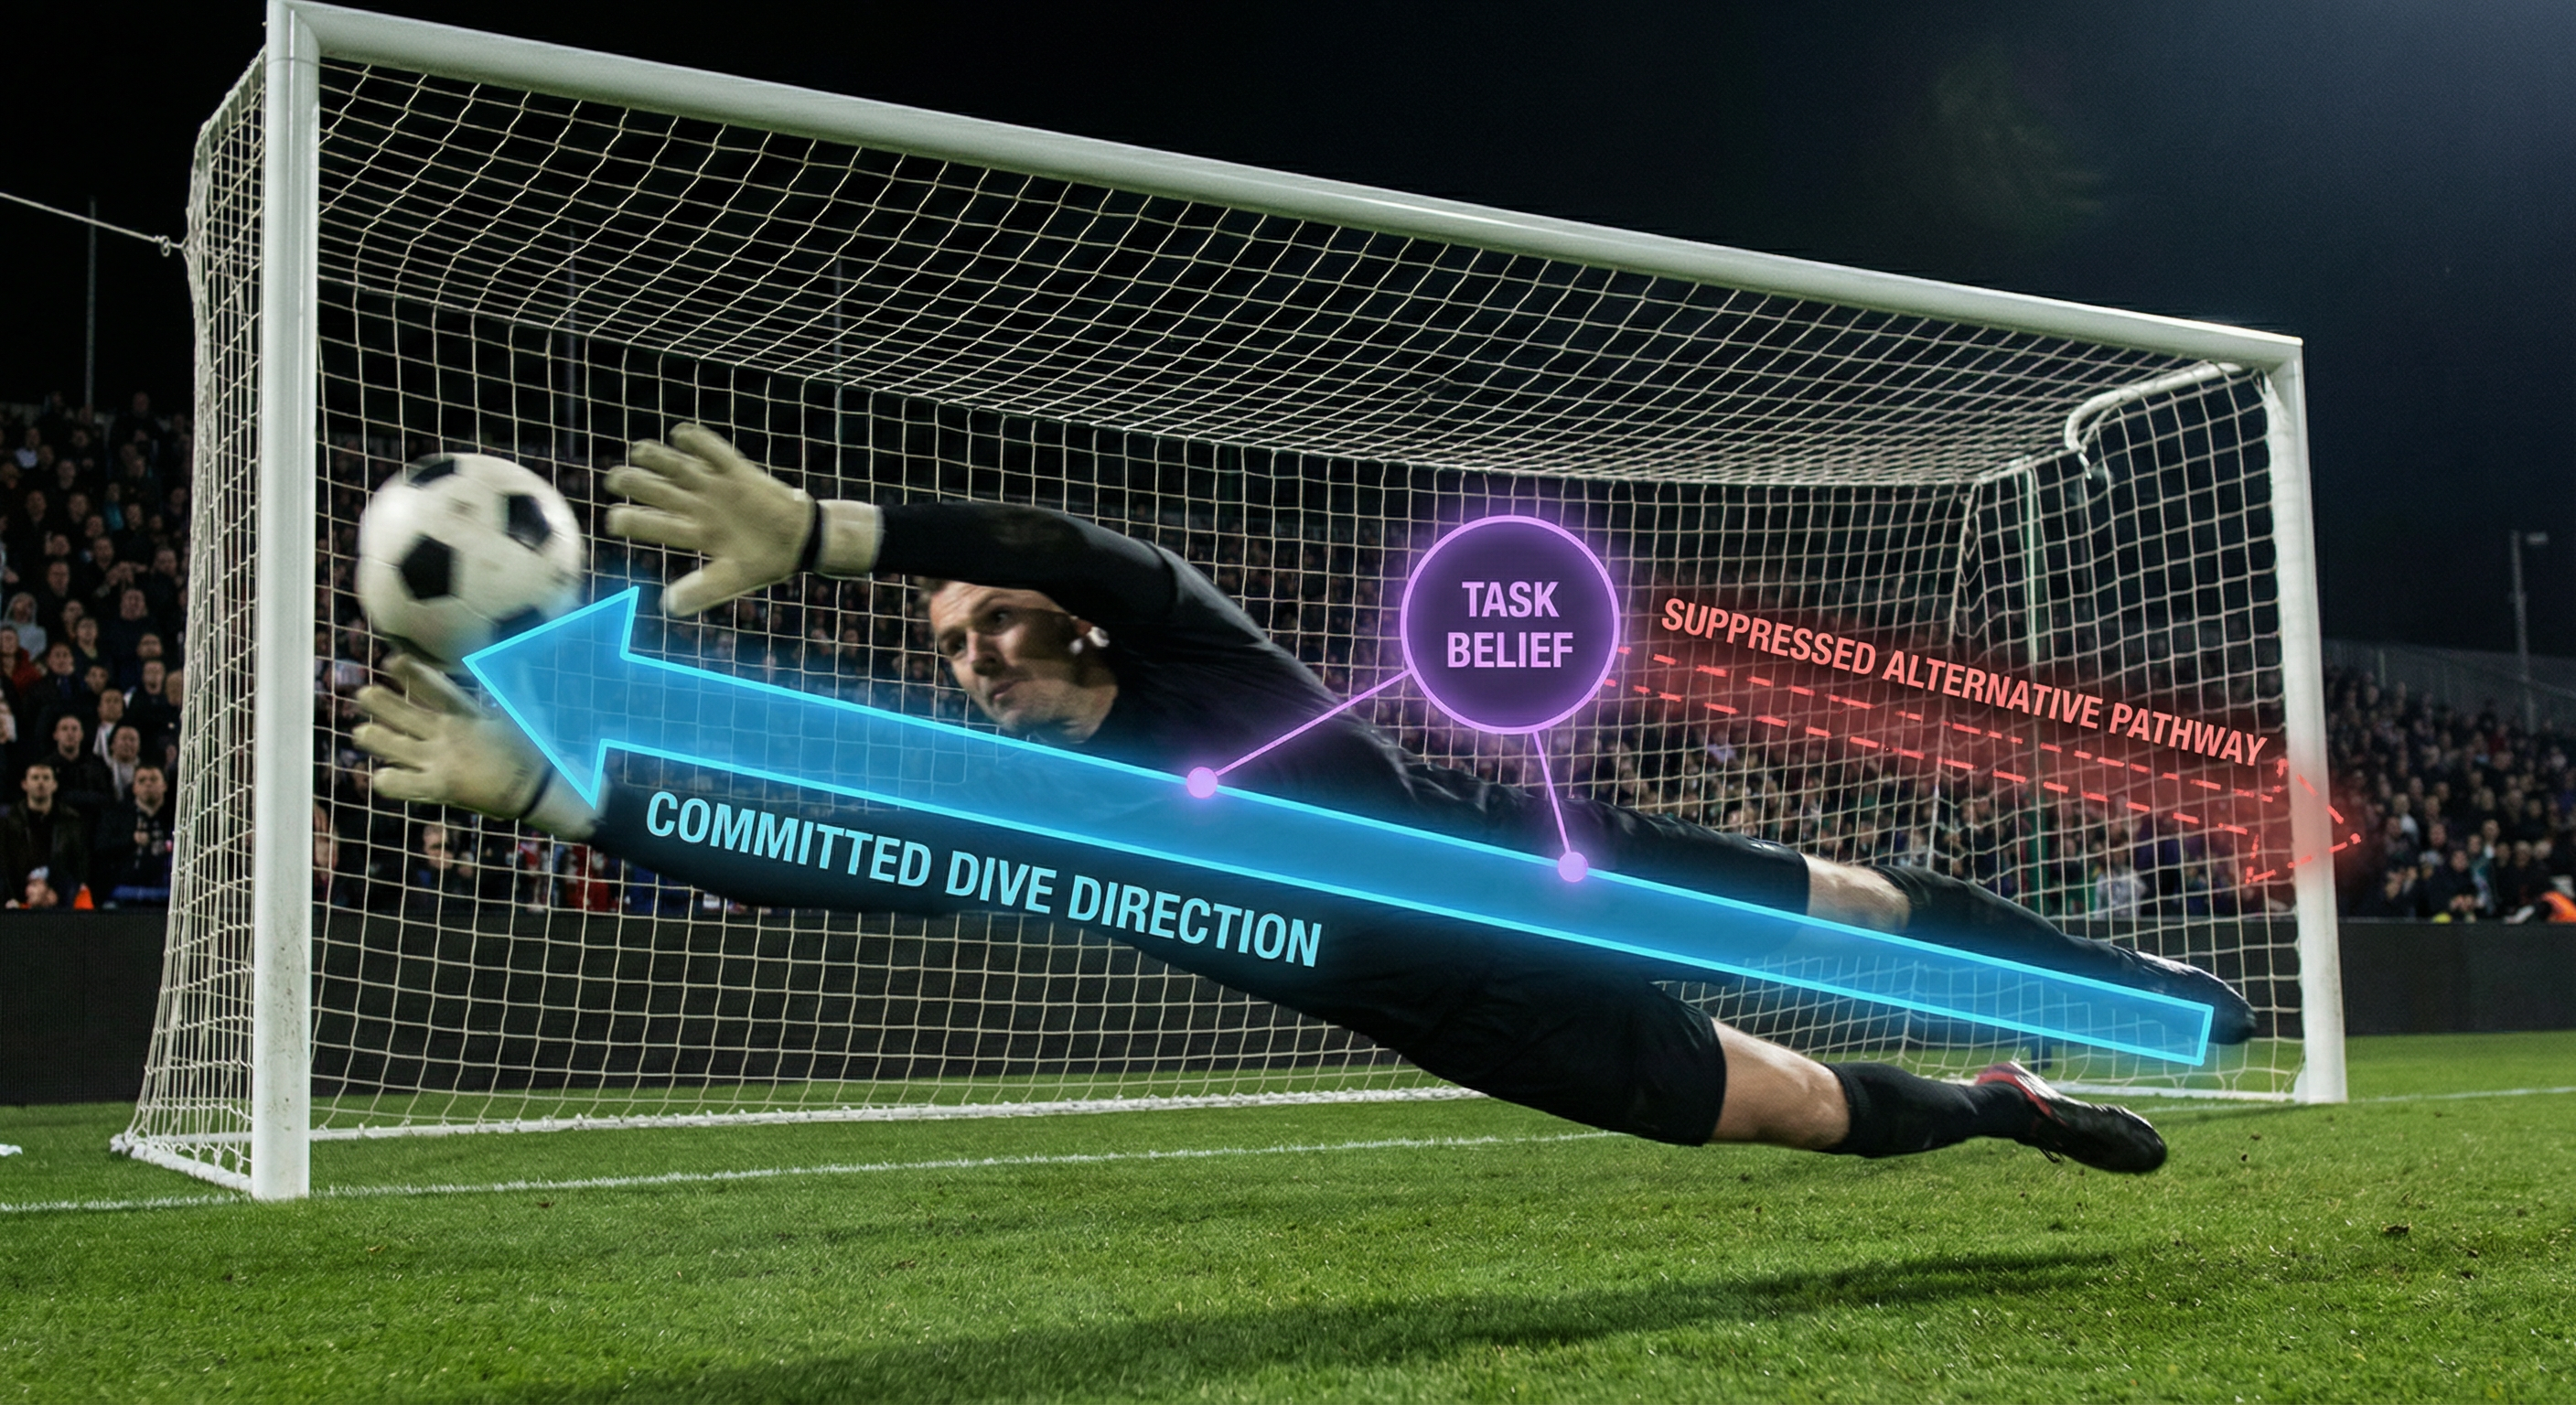
\includegraphics[width=\textwidth]{figures/keeper_motor_pathways.png}
\caption{\textbf{The goalkeeper's shared motor subspace.} A goalkeeper mid-dive illustrating the committed dive direction (blue arrow, engaged motor pathway) and the suppressed alternative (red dashed arrow). The ``Task Belief'' node (purple) represents the prefrontal gain modulation signal that selects between competing motor programmes that share the horizontal dive subspace. Once the motor programme is broadcast, sensory updates (e.g., seeing the ball go the other way) cannot override the committed response. Conceptual illustration; neural pathways are schematic.}
\label{fig:photo_keeper}
\end{figure*}

% ============================================================
\section{Introduction}

Every penalty taker has heard the advice: \emph{decide where you're going to shoot, and don't change your mind}.
The intuition is universal in coaching---being ``of two minds'' at the penalty spot costs you accuracy, power, or both.
But what is the mechanism?
Why should entertaining a second option degrade the execution of the first?
The soccer penalty kick distils the complexity of sport into a single confrontation.
The striker, standing 12 yards from goal, must place the ball past a goalkeeper who has approximately 500--600\,ms from foot-to-ball contact to the ball crossing the goal line \citep{vanderkamp2018goalkeeping}.
A goalkeeper's full-stretch dive requires 600--1000\,ms to execute, meaning that purely reactive goalkeeping is geometrically impossible for well-struck shots to the corners \citep{dicks2010anticipation}.
This temporal asymmetry forces the goalkeeper to act on anticipatory cues from the striker's body---run-up angle, plant-foot position, hip rotation, and kicking-leg trajectory---rather than on the ball's flight path \citep{diaz2012anticipating,lopes2014predicting}.

The result is a high-stakes perceptual-motor guessing game that has attracted analysis from economics \citep{palacioshuerta2003minimax,chiappori2002testing}, psychology \citep{bareli2007action,wilson2009anxiety}, biomechanics \citep{diaz2012anticipating}, and perception science \citep{wood2015quiet}.
Game-theoretic analysis suggests professional kickers and goalkeepers approximate minimax equilibrium play, randomising across directions such that neither player can improve by unilaterally changing strategy \citep{palacioshuerta2003minimax,chiappori2002testing}.
Yet the neurobiological mechanisms that actually \emph{implement} these decisions---the neural representations that guide anticipation, categorisation, and motor commitment---have received comparatively little attention.
In particular, the familiar coaching intuition that being ``of two minds'' is costly has lacked a mechanistic explanation grounded in how the brain actually organises competing action plans.

In this paper I propose that a recent discovery in systems neuroscience offers a surprisingly natural framework for understanding the penalty kick duel---and, specifically, for explaining \emph{why} indecision has a neural cost.
I then confront five of those predictions with publicly available penalty kick data, finding support for sequential-effect predictions but null results for several others---a pattern that clarifies where this framework adds value and where its limits lie.

\subsection{Compositional Tasks and Shared Subspaces}

Tafazoli et al.\ (\citeyear{tafazoli2026compositional}) trained macaque monkeys to flexibly switch between three categorisation tasks that were compositionally related---each task could be decomposed into a sensory subtask (categorise by colour or shape) and a motor subtask (respond on axis~1 or axis~2).
Recording from 1,081 neurons across five brain regions, they found that:

\begin{enumerate}
    \item The same \emph{subspaces} of neural activity represented colour category and motor response across tasks that shared those components.
    \item Information was processed \emph{sequentially}: sensory subspace encoding preceded motor subspace encoding by $\sim$63\,ms, with a task-specific transformation mapping sensory representations onto the correct motor output.
    \item A ``task belief'' signal, maintained in prefrontal cortex, acted as a gain modulator---amplifying representations in task-relevant subspaces and suppressing task-irrelevant dimensions.
    \item Task history effects persisted across intervening task blocks, biasing the animal's belief about the current task.
\end{enumerate}

The key computational trade-off: shared subspaces enable compositionality and generalisation, but they create \emph{interference} when two tasks compete for the same motor output channel.
These findings sit within a broader dynamical-systems perspective on motor control \citep{shenoy2013cortical} and extend models of urgency-gated commitment in action selection \citep{thura2014urgency,cisek2010neural}.

\subsection{The Penalty Kick as a Compositional Task}

I propose that both the goalkeeper and the striker face compositional task structures with shared subspaces, and that understanding the geometry of this sharing reveals why being ``of two minds'' is costly---why certain deception strategies work, why goalkeepers exhibit action bias, and why pre-commitment is advantageous for strikers.
The remainder of this paper is organised as follows: Section~2 maps the subspace framework onto the penalty kick; Section~3 derives seven predictions; Section~4 tests five of them empirically; Section~5 integrates the results with existing accounts; Section~6 offers a critical self-assessment; Section~7 proposes targeted experiments; and Section~8 concludes.

% ============================================================
\section{Mapping the Framework}

\subsection{The Goalkeeper's Task Battery}

The goalkeeper's decision space decomposes into sensory categorisation (``which way is the ball going?'') and motor response (``which way do I dive?''):

\begin{itemize}
    \item \task{Dive Left}: categorise striker cues $\rightarrow$ respond on horizontal axis (leftward push-off)
    \item \task{Dive Right}: categorise striker cues $\rightarrow$ respond on horizontal axis (rightward push-off)
    \item \task{Stay/Go Low}: categorise striker cues $\rightarrow$ respond on vertical axis (collapse or stand)
\end{itemize}

Critically, \task{Dive Left} and \task{Dive Right} share a motor subspace---both require explosive lateral push-off, hip rotation, and arm extension in the horizontal plane.
This is analogous to the S1 and C1 tasks in \citet{tafazoli2026compositional}, which shared axis~1 but required different sensory categorisations.
\task{Stay/Go Low} engages a fundamentally different motor programme---vertical collapse, centre-of-mass lowering---analogous to the C2 task on axis~2 (Figure~\ref{fig:mapping}).

\begin{figure*}[t]
\centering
\includegraphics[width=\textwidth]{figures/fig1_task_mapping.png}
\caption{\textbf{Mapping from monkey categorisation tasks to the penalty kick.}
\textbf{Left:} The three compositional tasks from \citet{tafazoli2026compositional}. S1 and C1 share axis~1 (orange bracket); C1 and C2 share colour categorisation (blue bracket).
\textbf{Right:} Proposed penalty kick mapping. Dive Left and Dive Right share the horizontal motor axis (red bracket). Stay/Go Low uses a different motor programme, analogous to C2's unique axis.}
\label{fig:mapping}
\end{figure*}

\subsection{The Striker's Task Battery}

The striker likewise faces compositional choices:

\begin{itemize}
    \item \task{Power Far Post}: strike through ball with high force, wide angle
    \item \task{Placement Near Post}: strike through ball with controlled force, tight angle
    \item \task{Chip}: scoop under the ball---entirely different kicking mechanics
\end{itemize}

\task{Power} and \task{Placement} share a motor subspace (striking \emph{through} the ball) but differ in force calibration and angular parameters.
The \task{Chip} uses a different motor subspace (scooping \emph{under} the ball), akin to a cross-axis switch (Figure~\ref{fig:photo_striker}).

\begin{figure*}[t]
\centering
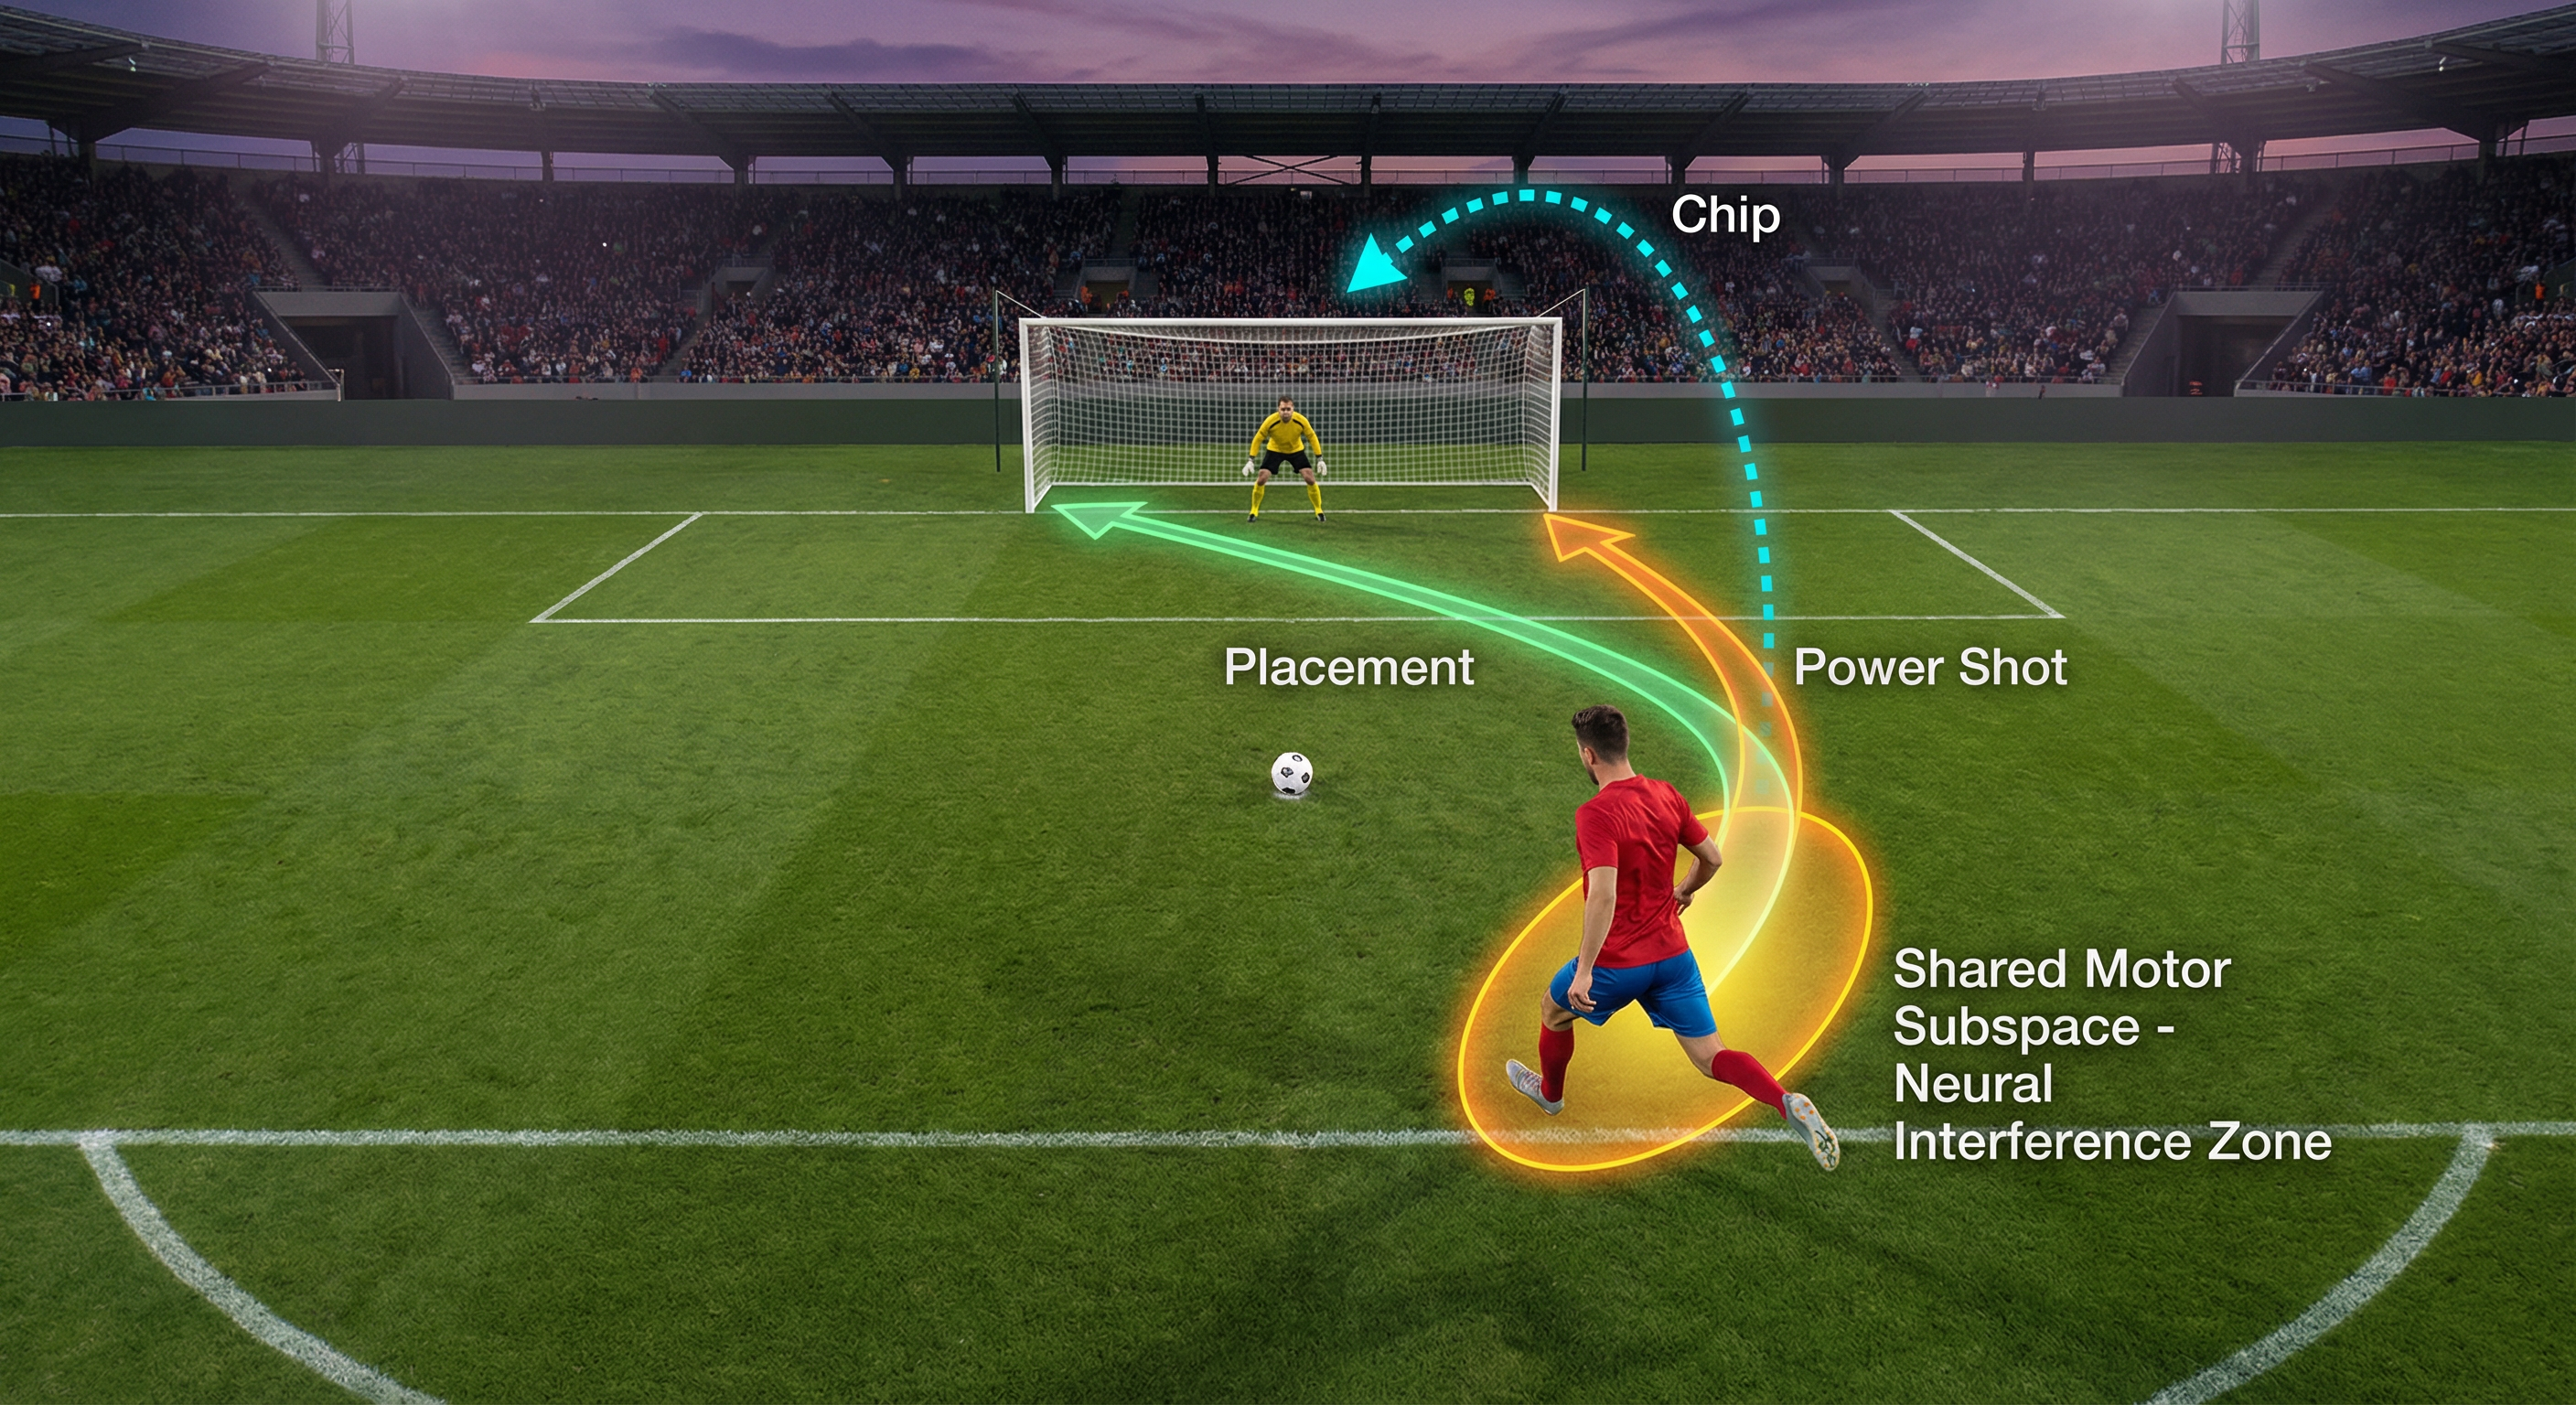
\includegraphics[width=\textwidth]{figures/striker_shared_subspace.png}
\caption{\textbf{The striker's compositional motor subspaces.} The ``Power Shot'' (orange) and ``Placement'' (green) share a motor subspace---both involve striking \emph{through} the ball---creating an interference zone where competing motor programmes degrade each other. The ``Chip'' (cyan, dotted) uses a fundamentally different motor programme (scooping under the ball), analogous to a cross-axis response with minimal interference. Conceptual illustration.}
\label{fig:photo_striker}
\end{figure*}

% ============================================================
\section{Predictions}

\subsection{Prediction 1: Within-Axis Interference Exceeds Cross-Axis Interference}

The core finding of \citet{tafazoli2026compositional} is that tasks sharing a motor response axis create persistent interference, whereas cross-axis switches are detected within 3--6 trials.

\textbf{Applied to the goalkeeper:} A deceptive run-up that feints left-then-goes-right (within the horizontal axis) should be harder to overcome than a fake suggesting a low shot that actually goes high (cross-axis).
Once the goalkeeper's motor system has begun loading the horizontal dive programme, re-directing to the opposite direction requires updating within a shared subspace.
Switching from a horizontal dive to a vertical collapse engages a different motor subspace entirely and should permit faster correction.

\subsection{Prediction 2: Task History Ghosts Across Successive Kicks}

Tafazoli et al.\ found that task belief persisted through an intervening block of a different task---the C1$\rightarrow$C2$\rightarrow$C1 sequence produced better performance than S1$\rightarrow$C2$\rightarrow$C1.

\textbf{Applied to a shootout:} If a goalkeeper dove left on kick~\#3, was presented with a different situation on kick~\#4, the framework predicts a residual bias toward diving left on kick~\#5.
This prediction runs counter to the gambler's fallacy---the well-documented tendency to expect alternation after repeated outcomes \citep{misirlisoy2014asymmetric}---but is consistent with the neural data showing persistent biases toward recent actions.

\begin{keeperbox}
\textbf{Speculative training cue:} After diving left, the framework suggests that the brain may maintain a residual pull toward left. Mentally rehearsing the \emph{opposite} direction during the walk-back to centre could, hypothetically, serve as a corrective.
\end{keeperbox}

\begin{strikerbox}
\textbf{Speculative training cue:} The neural-ghost hypothesis predicts that a goalkeeper's dive direction from \emph{two kicks ago} may be a better predictor of their next dive than the immediately preceding kick, because the intervening kick may not fully overwrite the earlier task representation.
\end{strikerbox}

\subsection{Prediction 3: The 63\,ms Transformation Window Is Exploitable}

The $\sim$63\,ms gap between sensory categorisation and motor commitment defines a temporal window in which information has been loaded into the sensory subspace but has not yet transformed into the motor subspace.

\textbf{Applied to the striker:} The stutter-step or hesitation run-up may exploit exactly this window.
By presenting body cues that load ``going right'' into the goalkeeper's sensory subspace, then altering direction, the striker catches the goalkeeper mid-transformation.
This reframes the biomechanical ``point of no return'' literature \citep{vanderkamp2018goalkeeping} in neural terms: the point of no return may be a gradient reflecting the progressive sensory-to-motor transformation, not a single threshold (Figure~\ref{fig:photo_transform}).

\begin{figure*}[t]
\centering
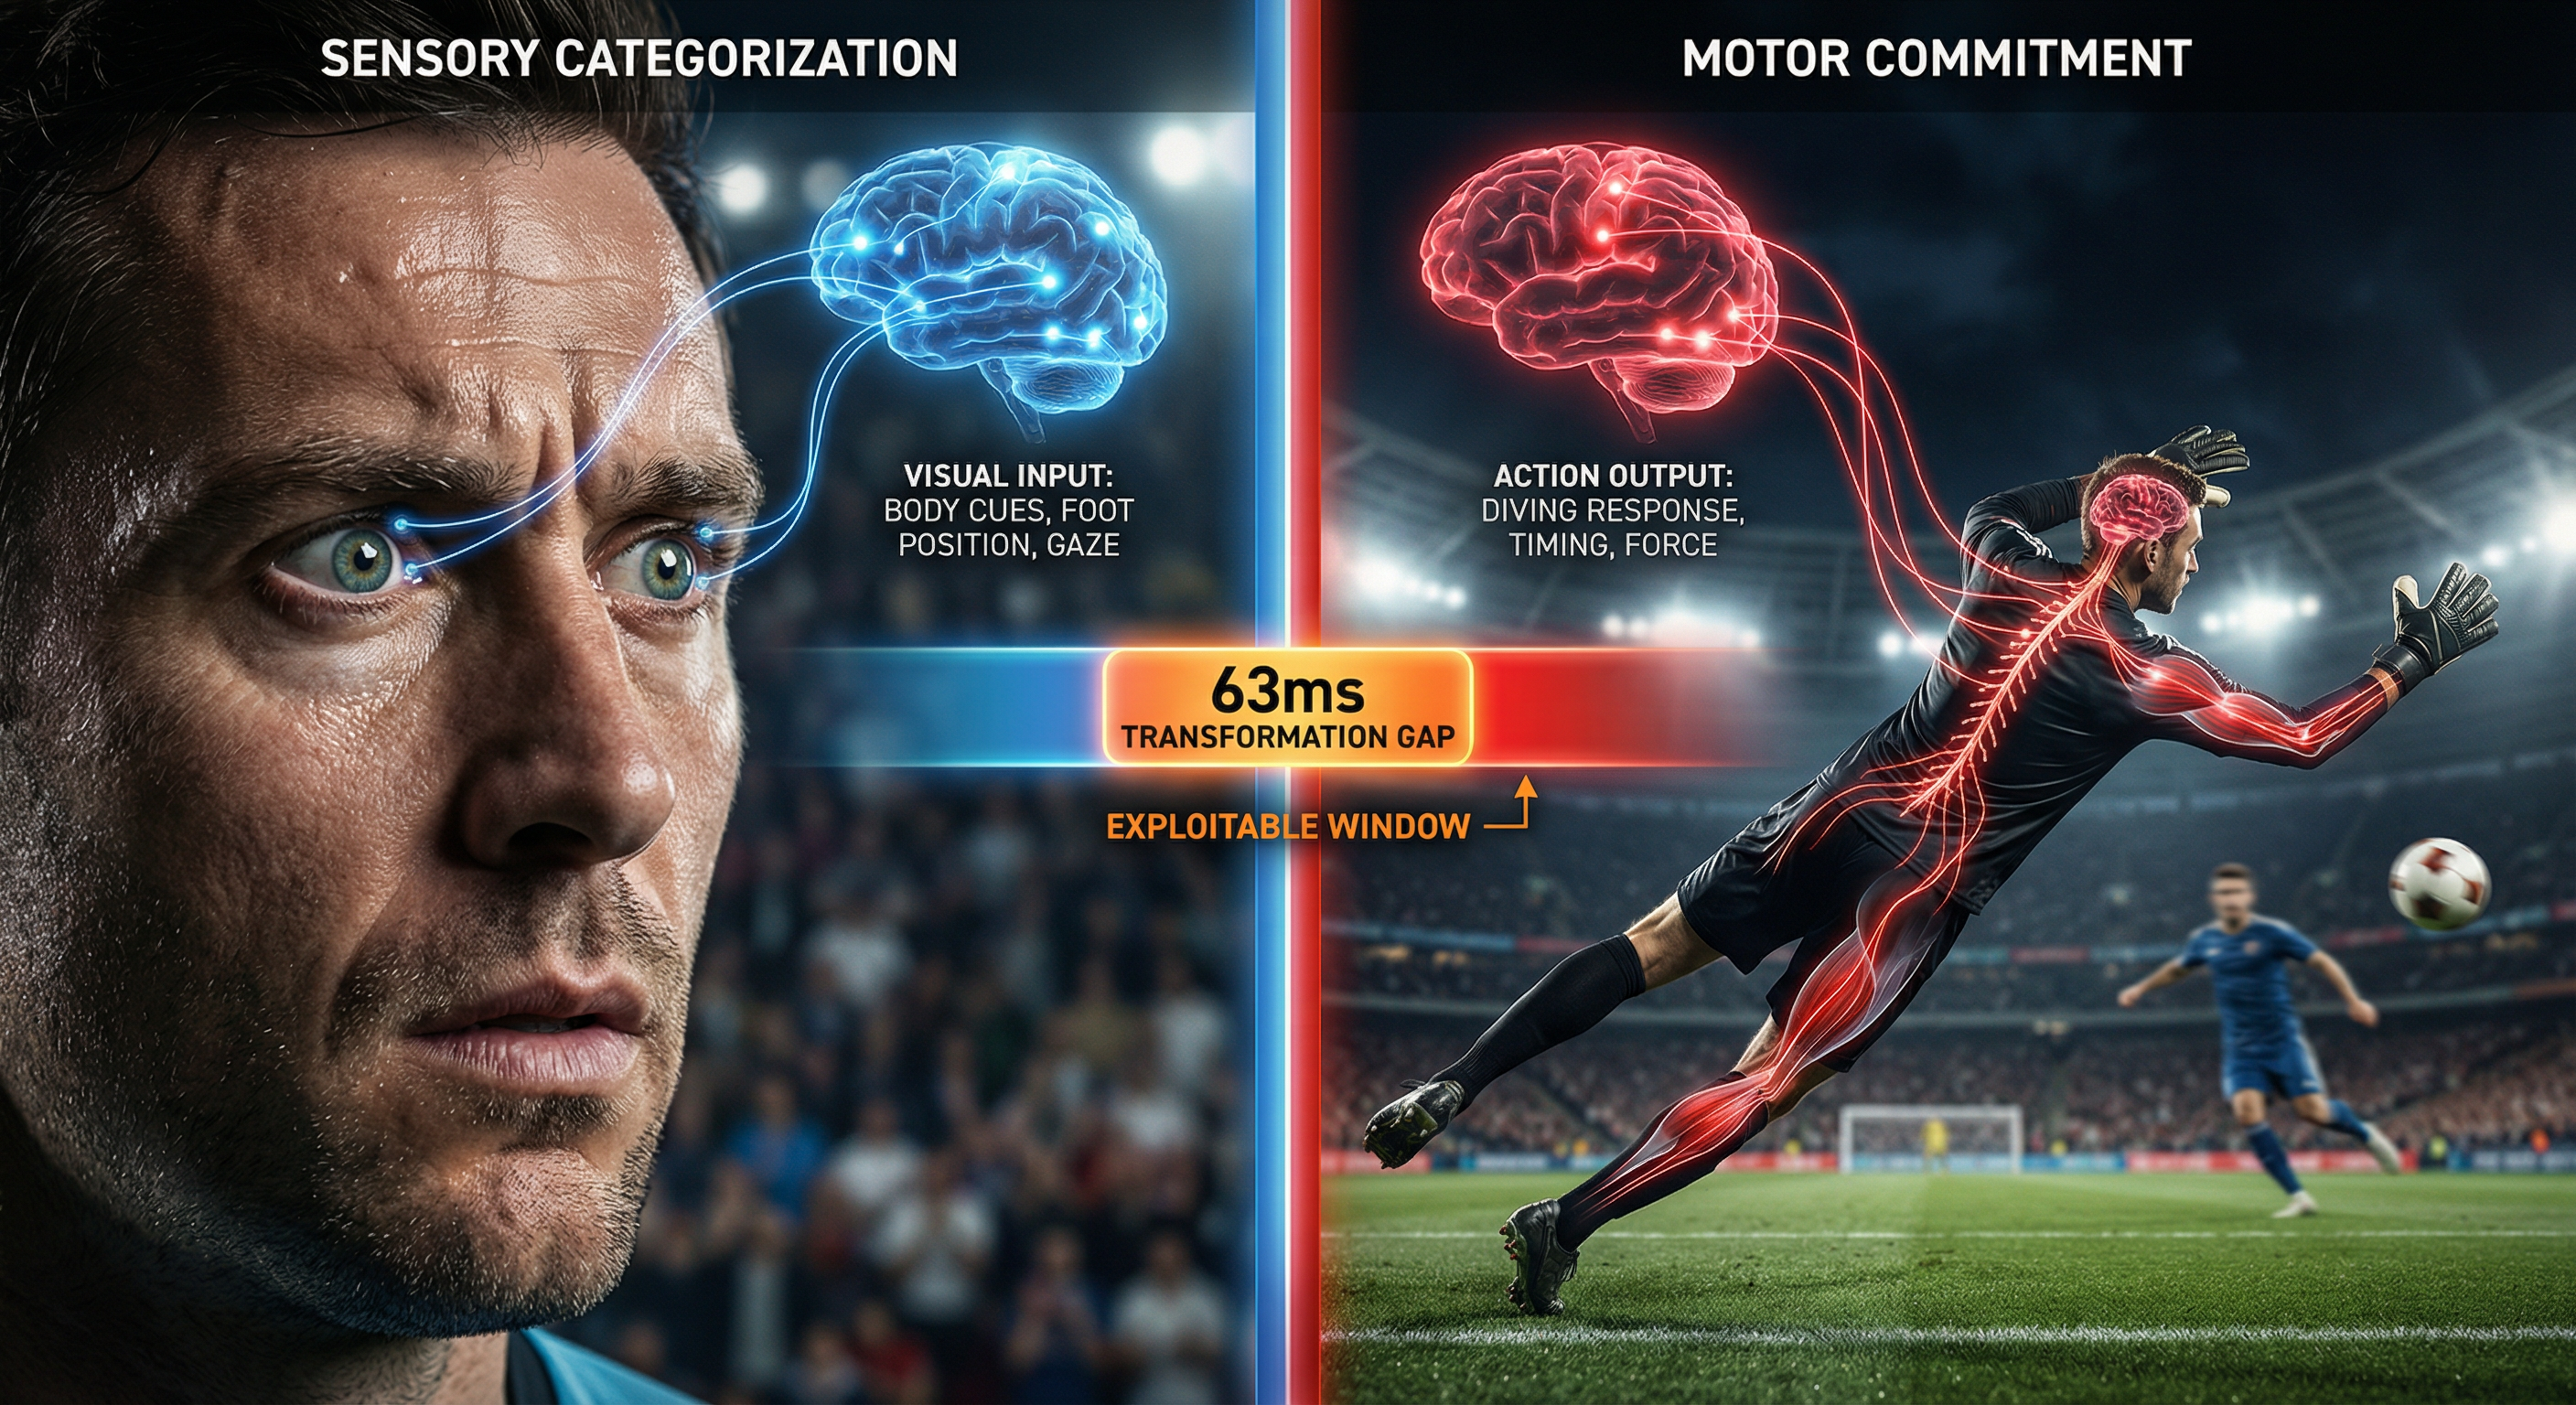
\includegraphics[width=\textwidth]{figures/transformation_window.png}
\caption{\textbf{The 63\,ms sensory-motor transformation gap.} \textbf{Left:} The goalkeeper during sensory categorisation---reading the striker's body cues with visual input streaming to prefrontal cortex (blue pathways). \textbf{Right:} 63\,ms later, motor commitment has been initiated and broadcast across the motor system (red pathways). The orange bar highlights the exploitable transformation window. Conceptual illustration; timing based on \citet{tafazoli2026compositional}.}
\label{fig:photo_transform}
\end{figure*}

\subsection{Prediction 4: Gain Modulation Creates Paradoxical Expertise Blind Spots}

The compression index (CPI) in \citet{tafazoli2026compositional} shows that task-relevant stimulus dimensions are amplified while irrelevant dimensions are suppressed.
Expert goalkeepers have learned that hip orientation is the most reliable predictor of shot direction \citep{diaz2012anticipating,lopes2014predicting}.

The framework predicts that this expertise-driven gain modulation should paradoxically create blind spots.
As the goalkeeper's neural system upweights hip kinematics, it simultaneously downweights less reliable cues such as gaze direction \citep{wood2015quiet}.
A deceptive gaze fixation may therefore be \emph{more} effective against experts who have stronger gain modulation.

\begin{keeperbox}
\textbf{Speculative training cue:} If gain modulation suppresses gaze-direction cues, periodically training with deliberate attention to ``suppressed'' channels (gaze, shoulder angle) may help prevent over-compression of potentially informative dimensions.
\end{keeperbox}

\begin{strikerbox}
\textbf{Speculative training cue:} Keeping hips neutral as long as possible, then rotating late, may exploit the goalkeeper's compressed gaze channel---the high-gain hip channel receives information too late for correction.
\end{strikerbox}

\subsection{Prediction 5: Keeper Centrality Maximises Striker Interference}

If the goalkeeper stays central and commits late, the striker is forced to remain ``of two minds''---maintaining both \task{Power Far Post} and \task{Placement Near Post} in parallel.
Because these share a motor subspace, the interference degrades both action plans simultaneously.
This provides a neural-level explanation for why goalkeepers who commit late perform better \citep{noelgomez2021interplay} and a mechanistic complement to the action bias paradox \citep{bareli2007action}: staying central may \emph{actively degrade the striker's motor execution} by forcing them to be of two minds for longer, maximising shared-subspace interference.

\subsection{Prediction 6: Pre-Commitment Reduces Interference, Not Reaction Time}

Strikers who pre-decide where to shoot score more frequently than those who react to the goalkeeper \citep{dicks2010anticipation,noelgomez2021interplay}, and late alterations of kick direction increase errors and reduce accuracy \citep{vanderkamp2006field,noel2015method}.
The standard explanation invokes reaction time limitations.

The subspace framework offers a different account: a pre-committed striker is of \emph{one} mind---running a single task with no shared-axis competition, analogous to C2, which uses a unique response axis and is executed accurately from trial~1.
A reactive striker is of \emph{two} minds---running the equivalent of C1 after an S1 block, with maximum shared-axis interference.
The advantage of pre-commitment is not speed but \emph{motor purity}: being of one mind means a cleaner motor programme (Figure~\ref{fig:precommit}).

\begin{figure}[t]
\centering
\includegraphics[width=\columnwidth]{figures/fig5_precommit.png}
\caption{\textbf{Pre-commitment reduces motor interference.}
Simulated shot-quality distributions for pre-committed (green) versus reactive (red) penalty kicks. Pre-committed shots cluster tightly; reactive shots are dispersed, reflecting contamination between competing motor programmes. Ellipses show 2-SD spread.}
\label{fig:precommit}
\end{figure}

\begin{strikerbox}
\textbf{Speculative training cue:} ``Pick a side and commit'' may be not merely a motivational platitude but a prescription for being of \emph{one} mind---reducing shared-subspace interference and yielding a cleaner motor programme.
\end{strikerbox}

\subsection{Prediction 7: The Motor Broadcast Lock-In}

Motor representations were shared across \emph{all} recorded brain regions in \citet{tafazoli2026compositional}, while sensory representations were localised to prefrontal cortex.
This ``motor broadcast'' means that once a motor programme initiates, it is committed globally.

For the goalkeeper, this predicts a dissociation: they can visually register a change in shot direction (sensory update, local and fast) but cannot modify their motor response (global and committed)---producing the characteristic experience of ``seeing'' the ball go the other way while being unable to alter the dive.

% ============================================================
\section{Empirical Tests}
\label{sec:empirical}

I tested Predictions 1, 2, 4, 5, and 6 against two publicly available penalty kick datasets.
Predictions 3 and 7 require millisecond-level kinematic or neural data that these behavioural datasets cannot provide.

\subsection{Data and Analysis Plan}

\textbf{Datasets.} Two publicly available datasets were used:
\begin{enumerate}
    \item \textbf{Multi-league penalty dataset} ($N = \PredOneNTotal$ penalties, 2020--2025): sourced from Kaggle, covering penalties from multiple national leagues (predominantly Portugal, with additional European leagues). Variables include kicker shot direction (L/C/R), goalkeeper dive direction (L/C/R), kicker dominant foot, binary outcome (goal/no goal), goalkeeper name, and match context (country, minute, score).
    \item \textbf{Bundesliga dataset} ($N = \PredFourNTotal$ penalties, 1963--2017): a comprehensive record of Bundesliga penalties with outcome (goal, save, miss type), match date, minute, goal difference at time of kick, goalkeeper and penalty-taker identities, club affiliations, and experience (seasons).
\end{enumerate}

\textbf{Operational definitions.}
A ``goal'' is a scored penalty; ``non-goal'' includes goalkeeper saves \emph{and} misses (off-target, post, crossbar).
Goalkeeper ``experience'' is operationalised as the number of Bundesliga seasons in which they faced at least one penalty.
``Same-goalkeeper sequences'' in the multi-league dataset are defined as consecutive rows where the goalkeeper name and country both match, providing a proxy for same-match or same-competition appearances (note: this is an imperfect proxy and results should be interpreted cautiously).
``Foot congruence'' classifies a shot as ``natural'' (cross-body: right foot to left, or left foot to right) versus ``unnatural'' (same-side).

\textbf{Statistical approach.}
All analyses were conducted in Python (scipy, statsmodels, pandas); code, data, and a reproducible \texttt{Makefile} are available at the project repository.
Because these are exploratory observational checks rather than confirmatory hypothesis tests, I report both \emph{p}-values and effect sizes with 95\% confidence intervals where feasible.
The primary analyses use chi-squared tests, Fisher exact tests, binomial tests, and logistic regression.
Where penalties are nested within matches or goalkeepers, I note the clustering but acknowledge that the sample sizes generally preclude mixed-effects models; results should be treated as exploratory.

\textbf{Prediction--measurement alignment.}
Table~\ref{tab:measurement} maps each prediction to its underlying mechanism and the minimal measurement required, clarifying which predictions can and cannot be tested with the available data.

\begin{table}[t]
\centering
\caption{Prediction--measurement alignment.}
\label{tab:measurement}
\small
\begin{tabular}{@{}p{0.7cm}p{2.2cm}p{2.2cm}p{1.2cm}@{}}
\toprule
\textbf{P\#} & \textbf{Mechanism} & \textbf{Min.\ measure} & \textbf{Data?} \\
\midrule
1 & Motor subspace interference & Kinematic dive correction & No \\
\addlinespace
2 & Task-history ghost & Choice direction sequence & \textbf{Yes} \\
\addlinespace
3 & Sensory$\rightarrow$motor transform & ms-level timing & No \\
\addlinespace
4 & Gain modulation & Deceptive cue response & Partial \\
\addlinespace
5 & Shared-axis interference & Shot quality metrics & No \\
\addlinespace
6 & Motor purity & Internal commitment state & Partial \\
\addlinespace
7 & Motor broadcast & Neural / EMG data & No \\
\bottomrule
\end{tabular}
\end{table}

\subsection{Prediction 1: Within- vs.\ Cross-Axis Interference}

\textbf{Method.} I classified each Kaggle penalty by the relationship between the kicker's shot direction and the goalkeeper's dive direction: \emph{match} (same direction), \emph{within-axis mismatch} (both on the horizontal axis: kicker shoots left, keeper dives right or vice versa), or \emph{cross-axis mismatch} (one horizontal, one centre).
The framework predicts lower conversion (i.e., more saves) for within-axis mismatches than cross-axis mismatches, because the goalkeeper should recover more easily from a cross-axis error.

\textbf{Results.} Conversion rates were $\PredOneConvWithin$ for within-axis mismatches ($n = \PredOneNWithin$) and $\PredOneConvCross$ for cross-axis mismatches ($n = \PredOneNCross$), with $\PredOneConvMatch$ for matches ($n = \PredOneNMatch$).
The Fisher exact test comparing within- and cross-axis mismatches was not significant (OR $= \PredOneFisherOR$, $p = \PredOneFisherP$).
The dominant effect was match versus mismatch ($\chi^2 = \PredOneChiSq$, $p < 0.001$): when the goalkeeper dived the wrong way, the ball almost always went in regardless of axis (Figure~\ref{fig:emp_pred1}).

\begin{figure}[t]
\centering
\includegraphics[width=\columnwidth]{figures/empirical_pred1_conversion_by_mismatch.png}
\caption{\textbf{Prediction 1: conversion rate by mismatch type.}
Both within-axis and cross-axis mismatches produce near-ceiling conversion rates ($>95\%$), vastly exceeding the match condition. The prediction of differential interference between mismatch types is not supported.}
\label{fig:emp_pred1}
\end{figure}

\textbf{Interpretation.}
The null result likely reflects a floor effect on the goalkeeper's ability to save: when the keeper dives the wrong direction at all, recovery is essentially impossible within the $\sim$500\,ms flight time, regardless of whether the error was within-axis or cross-axis.
The subspace-interference prediction concerns the \emph{speed of motor re-direction}, which is invisible in binary outcome data.
Testing this prediction properly requires kinematic measures of dive correction---force-plate data, motion capture, or at minimum video-based reaction time analysis.

\subsection{Prediction 2: Sequential Effects}
\label{sec:pred2}

\textbf{Method.} Using the Bundesliga dataset, I identified matches containing two or more penalties ($n = \PredTwoNMultiMatches$ matches, $\PredTwoNPairs$ consecutive pairs) and tested whether the outcome of penalty $n-1$ predicted the outcome of penalty $n$ within the same match.
Separately, using the Kaggle dataset, I identified same-match goalkeeper appearances ($n = \PredTwoKaggleNSameMatch$ pairs) and tested whether goalkeepers repeated their dive direction more than expected by chance.

\textbf{Results.} Goals were significantly more likely after a previous goal ($\PredTwoGoalAfterGoal$, $n = \PredTwoNAfterGoal$) than after a previous non-goal ($\PredTwoGoalAfterSave$, $n = \PredTwoNAfterSave$; $\chi^2 = \PredTwoChiSq$, $p = \PredTwoChiP$; risk difference $= \PredTwoRiskDiff$, 95\% CI $[\PredTwoRiskDiffCILo, \PredTwoRiskDiffCIHi]$).
A logistic regression controlling for goal difference, match minute, and home advantage confirmed the sequential effect ($\beta_{\text{prev\_goal}} = \PredTwoLogitCoef$, $p = \PredTwoLogitP$).
The effect was present for both previous saves and previous misses, though the small number of miss pairs limits fine-grained disaggregation ($\PredTwoGoalAfterSaveOnly$ after saves, $\PredTwoGoalAfterMiss$ after misses).
In the multi-league data, goalkeepers repeated their dive direction $\PredTwoKaggleRepeatRate$ of the time across consecutive same-goalkeeper penalties ($n = \PredTwoKaggleNSameMatch$ pairs), significantly above the $33\%$ expected by chance ($p = \PredTwoKaggleBinomP$, binomial test; Figure~\ref{fig:emp_pred2}).

\begin{figure}[t]
\centering
\includegraphics[width=\columnwidth]{figures/empirical_pred2_sequential.png}
\caption{\textbf{Prediction 2: sequential effects.} \textbf{A.} Bundesliga: goals are significantly more likely after a previous goal than after a non-goal ($p = \PredTwoChiP$). Error bars show 95\% Wilson CIs. \textbf{B.} Multi-league data: goalkeepers repeated their dive direction $\PredTwoKaggleRepeatRate$ of the time across consecutive same-goalkeeper penalties ($p = \PredTwoKaggleBinomP$).}
\label{fig:emp_pred2}
\end{figure}

\textbf{Interpretation.}
This is the most striking result.
Despite the fact that these are in-game penalties (not shootouts), separated by substantial stretches of play, a significant sequential dependency emerges: goals beget goals, and goalkeepers strongly repeat their dive direction.
This is consistent with the ``task-history ghost'' from \citet{tafazoli2026compositional}, where the prior task's representation persisted through an intervening block.
The result also runs counter to the gambler's fallacy---where goalkeepers have been shown to expect alternation in shootout contexts \citep{misirlisoy2014asymmetric}---and to the minimax prediction of serial independence \citep{palacioshuerta2003minimax}.
The controlled logistic regression suggests the effect is not fully explained by within-match score context.

However, alternative explanations exist and must be carefully weighed.
The goal-after-goal effect may partly reflect within-match psychological momentum \citep{jordet2009superstars}, a common penalty taker, or even selection bias (a team awarded multiple penalties may be dominant).
The goalkeeper repetition effect could reflect a strong side preference rather than a trial-to-trial sequential bias.
The small sample of consecutive same-goalkeeper pairs ($n = \PredTwoKaggleNSameMatch$) warrants particular caution.
Dedicated shootout data---where kicks are tightly sequenced and goalkeeper identity is constant---would provide a substantially stronger test \citep{jordet2008avoidance,jordet2009temporal}.

\subsection{Prediction 4: Expertise Blind Spots}

\textbf{Method.} Using the Bundesliga dataset ($N = \PredFourNTotal$), I operationalised goalkeeper expertise as the number of Bundesliga seasons in which they faced penalties and modelled save rate as a function of experience (linear and quadratic logistic regression).

\textbf{Results.} Overall save rate was $\PredFourOverallSave$.
The linear term was non-significant ($\beta = \PredFourLinCoef$, $p = \PredFourLinP$) and the quadratic term showed a non-significant inverted-U peaking at $\PredFourPeakExp$ seasons ($\beta_{\text{quad}} = \PredFourQuadCoef$, $p = \PredFourQuadP$; likelihood-ratio test for the quadratic model: $\chi^2 = \PredFourLRChi$, $p = \PredFourLRP$; Figure~\ref{fig:emp_pred4}).

\begin{figure}[t]
\centering
\includegraphics[width=\columnwidth]{figures/empirical_pred4_expertise.png}
\caption{\textbf{Prediction 4: expertise and save rate.} Logistic regression of save rate on goalkeeper experience (seasons). A non-significant quadratic trend peaks at $\sim$$\PredFourPeakExp$ seasons, suggestive of but insufficient to confirm the expertise-blind-spot hypothesis.}
\label{fig:emp_pred4}
\end{figure}

\textbf{Interpretation.}
The data do not support or refute the expertise blind-spot prediction.
Season count is a coarse proxy for perceptual expertise, and save rate aggregates over heterogeneous shot types.
A proper test requires measuring expert versus novice goalkeepers' responses to deceptive versus non-deceptive stimuli in controlled conditions, isolating the gain-modulation mechanism.

\subsection{Prediction 5: Keeper Centrality}

\textbf{Method.} Using the Kaggle dataset, I compared conversion rates when goalkeepers stayed central ($n = \PredFiveNCentral$) versus dived ($n = \PredFiveNDive$).

\textbf{Results.} Conversion rates were $\PredFiveConvCentral$ (central) versus $\PredFiveConvDive$ (diving; Fisher exact $p = \PredFiveFisherP$; proportion $z$-test $p = \PredFiveZP$; Figure~\ref{fig:emp_pred5}).
With only $\PredFiveNCentral$ central penalties, the analysis is severely underpowered.

\begin{figure}[t]
\centering
\includegraphics[width=\columnwidth]{figures/empirical_pred5_centrality.png}
\caption{\textbf{Prediction 5: keeper centrality.} No difference in conversion rate between central and diving goalkeepers, but the central condition has only $n = \PredFiveNCentral$ cases.}
\label{fig:emp_pred5}
\end{figure}

\textbf{Interpretation.}
The null result is unsurprising given the tiny sample of central stays, which itself reflects the action bias documented by \citet{bareli2007action}.
The prediction concerns shot \emph{quality} degradation (velocity, accuracy), not just binary outcome.
Testing it requires shot-quality metrics as a function of goalkeeper commitment timing.

\subsection{Prediction 6: Pre-Commitment (Foot Congruence)}

\textbf{Method.} I used the kicker's dominant foot and shot direction to proxy pre-commitment: a right-footed kicker shooting left (cross-body) is executing the ``natural'' power-shot motor programme, plausibly reflecting a pre-committed plan; the reverse (shooting to the dominant-foot side) requires a less natural technique, plausibly reflecting a reactive adjustment. I compared conversion rates between natural-side ($n = \PredSixNNatural$) and unnatural-side shots ($n = \PredSixNUnnatural$).

\textbf{Results.} Conversion rates were $\PredSixConvNatural$ (natural) versus $\PredSixConvUnnatural$ (unnatural; Fisher exact $p = \PredSixFisherP$).
A logistic regression including goalkeeper-kicker side matching showed that the match variable dominated ($\beta = \PredSixLogitMatchCoef$, $p < 0.001$), while the foot-congruence variable was non-significant ($\beta = \PredSixLogitNatCoef$, $p = \PredSixLogitNatP$; Figure~\ref{fig:emp_pred6}).

\begin{figure}[t]
\centering
\includegraphics[width=\columnwidth]{figures/empirical_pred6_congruence.png}
\caption{\textbf{Prediction 6: foot congruence as pre-commitment proxy.} No significant difference between natural-side and unnatural-side kicks. The dominant predictor of conversion is whether the goalkeeper dived the correct way.}
\label{fig:emp_pred6}
\end{figure}

\textbf{Interpretation.}
Foot congruence is a weak proxy for pre-commitment.
Many factors beyond motor-programme interference determine whether a kicker shoots cross-body or same-side (tactical habit, the goalkeeper's expected dive, practice routines).
The framework's prediction concerns the \emph{internal} state of the kicker---whether they are running a single motor programme or two competing ones---which cannot be inferred from foot laterality alone.
Virtual-reality paradigms that experimentally manipulate the number of response options available to the kicker would provide a more direct test.

\subsection{Summary of Empirical Results}

\begin{table}[t]
\centering
\caption{Summary of empirical tests.}
\label{tab:empirical}
\small
\begin{tabular}{@{}p{1.8cm}p{2.8cm}p{2.0cm}@{}}
\toprule
\textbf{Prediction} & \textbf{Finding} & \textbf{Verdict} \\
\midrule
P1: Axis interference & Both mismatch types $\sim$95\% conversion & Not supported (floor effect) \\
\addlinespace
P2: Sequential effects & Goals predict goals; GK repeats side & \textbf{Supported} ($p < 0.01$) \\
\addlinespace
P4: Expertise blind spots & Non-significant quadratic trend & Inconclusive \\
\addlinespace
P5: Centrality & No difference ($n = 12$) & Underpowered \\
\addlinespace
P6: Pre-commit & No foot-congruence effect & Not supported (weak proxy) \\
\bottomrule
\end{tabular}
\end{table}

Table~\ref{tab:empirical} summarises the empirical findings.
The pattern is clear: one prediction receives significant support (sequential effects), while the others are either null or limited by the coarseness of available data.
This is informative rather than devastating.
The framework's predictions concern neural-level mechanisms (motor subspace interference, gain modulation, sensory-motor transformation timing) that are largely invisible in binary penalty outcome data.
The sequential-effects result is notable precisely because it is the prediction most naturally observable in behavioural data---task-history ghosts manifest as biases in choice direction, which \emph{is} recorded in penalty kick databases.

% ============================================================
\section{Integration with Existing Accounts}

Table~\ref{tab:integration} summarises how the shared-subspace framework relates to and extends existing analyses of the penalty kick.

\begin{table*}[t]
\centering
\caption{Integration of the shared-subspace framework with existing penalty kick accounts.}
\label{tab:integration}
\small
\begin{tabular}{@{}p{3.2cm}p{4.5cm}p{4.5cm}@{}}
\toprule
\textbf{Existing Account} & \textbf{Key Claim} & \textbf{Subspace Reinterpretation} \\
\midrule
Game Theory \citep{palacioshuerta2003minimax,chiappori2002testing} & Players randomise to approximate minimax equilibrium & Serial independence may break down via task-history ghosts (P2; empirically supported) \\
\addlinespace
Action Bias \citep{bareli2007action,bareli2009irrationality} & Goalkeepers dive too often due to regret asymmetry & Staying central may also maximise striker motor interference (P5; underpowered test) \\
\addlinespace
Perceptual Expertise \citep{mann2007perceptual} & Experts read anticipatory cues better & Expertise creates gain modulation that paradoxically suppresses some cues (P4; inconclusive) \\
\addlinespace
Quiet Eye / Attention \citep{wood2015quiet,wilson2009anxiety,wood2010moving} & Deceptive gaze exploits attentional capture; anxiety disrupts control & Gaze deception exploits a \emph{suppressed} dimension; anxiety may weaken gain modulation \\
\addlinespace
Pre-commitment \citep{dicks2010anticipation,vanderkamp2006field} & Fixed-target strategy is better; late alterations impair accuracy & Pre-commitment eliminates shared-subspace interference (P6; weak proxy) \\
\addlinespace
Point of No Return \citep{vanderkamp2018goalkeeping,thura2014urgency} & Discrete threshold for dive commitment & Continuous gradient of sensory$\rightarrow$motor transformation (P3; untested) \\
\bottomrule
\end{tabular}
\end{table*}

% ============================================================
\section{A Critical Self-Assessment}

\textbf{Species gap.}
The core evidence comes from macaque monkeys performing eye-movement categorisation tasks.
Penalty kicks involve whole-body ballistic movements under extreme time and social pressure.
The degree to which shared subspace architecture generalises from primate PFC saccadic responses to human cortical and subcortical motor control during sport is unknown.

\textbf{Task complexity.}
The monkey experiment involved three tasks with well-defined categories and fixed stimulus-response mappings.
A penalty kick involves continuous sensory input, self-generated body dynamics, opponent modelling, and emotional regulation.
The decomposition into discrete ``tasks'' with shared ``axes'' is a useful analogy but certainly an oversimplification.

\textbf{Timescale mismatch.}
The task-discovery dynamics in \citet{tafazoli2026compositional} unfold over 75+ trials.
A penalty shootout involves at most 5--10 kicks.
Whether task-history effects accumulate over such few ``trials'' is questionable---though the significant sequential effects in our in-game data (Section~\ref{sec:pred2}), where penalties are separated by long stretches of play, suggest that the neural ghost may be surprisingly persistent.

\textbf{Empirical record.}
Of five predictions tested, only one (sequential effects) received significant support.
While the null results are largely attributable to methodological limitations (floor effects, underpowered samples, weak proxies), a sceptic could reasonably conclude that the framework has little empirical traction in the domain.
I have attempted to be transparent about which null results reflect data limitations and which may reflect genuine failures of the predictions.

\textbf{The analogy itself.}
Mapping ``colour vs.\ shape categorisation'' onto ``hip kinematics vs.\ gaze direction,'' or ``axis~1 vs.\ axis~2'' onto ``dive left/right vs.\ stay central,'' involves interpretive choices.
Different mappings might yield different predictions.
This flexibility is simultaneously the framework's strength (wide applicability) and weakness (risk of \emph{post hoc} rationalisation).

% ============================================================
\section{Proposed Experiments}

The empirical tests in Section~\ref{sec:empirical} highlight a clear gap: the predictions that received null results are precisely those requiring kinematic or neural data rather than binary outcomes.
I propose six targeted experiments:

\begin{enumerate}
    \item \textbf{Within- vs.\ cross-axis recovery (P1):}
    Use motion-capture and force-plate data to measure goalkeeper recovery time after deceptive stimuli that redirect within the horizontal axis versus across axes.

    \item \textbf{Shootout sequential analysis (P2):}
    Re-analyse FIFA World Cup and Euro shootout databases to test kick-$n$-minus-2 predictions with full sequential structure.

    \item \textbf{Stutter-step timing (P3):}
    Manipulate the deceptive-cue-to-true-cue gap in a virtual-reality paradigm around the predicted $\sim$60\,ms transformation window.

    \item \textbf{Expert blind spots (P4):}
    Compare novice and expert goalkeepers' susceptibility to gaze deception. If gain modulation increases with expertise, experts should be \emph{more} susceptible.

    \item \textbf{Shot quality under uncertainty (P5):}
    Measure shot velocity and placement accuracy as a function of goalkeeper commitment timing, testing whether late-committing keepers degrade shot quality.

    \item \textbf{EEG lateralised readiness potential (P3, P7):}
    Record scalp EEG from goalkeepers performing anticipation tasks; the LRP onset should dissociate from perceptual categorisation.
\end{enumerate}

% ============================================================
\section{Concluding Remarks}

The penalty kick is not merely a guessing game.
It is a duel over who can force the other to be ``of two minds'' for longest---and who can resolve their own indecision first.
The goalkeeper wants to remain maximally ambiguous, forcing the striker to maintain two competing motor plans simultaneously; the striker wants to collapse their own task structure to a single, clean sensory-motor transformation.
Each player attempts to maximise the opponent's within-axis interference while minimising their own.

Of the seven predictions derived from \citet{tafazoli2026compositional}, one receives clear empirical support in observational data: the task-history ghost.
Goalkeepers repeat their dive direction well above chance, and goals beget goals---a sequential dependency inconsistent with minimax serial independence but consistent with persistent task-belief representations in prefrontal cortex.
The remaining predictions could not be adequately tested with binary outcome data but remain testable with kinematic and neural measures.

The familiar coaching advice---``pick a corner and commit; don't be of two minds''---may be not just motivational platitude but a prescription for neural hygiene.
Pre-commitment eliminates shared-subspace interference.
The resulting motor programme is pure, fast, and uncontaminated by the ghost of the road not taken.

Of course, the road from a monkey categorising coloured shapes to a footballer standing over a ball in a World Cup final is a long one.
But if the brain builds complex behaviour by composing shared representational subspaces---and the evidence suggests it does---then every competitive interaction between two brains is, at some level, a battle over whose subspaces interfere with whose.
Being ``of two minds'' is the cost of flexibility.
The penalty kick is simply where the stakes make that cost impossible to ignore.

% ============================================================
\section*{Acknowledgements}

I thank Sina Tafazoli, Timothy J.\ Buschman, and colleagues for making their data and code publicly available, and for producing research that is both rigorous and imaginatively stimulating.
I am grateful to the penalty kick research community, whose meticulous empirical work made the connections drawn here possible, and to the creators of the Kaggle and Bundesliga penalty kick datasets.

\textbf{Generative AI disclosure.}
This paper benefited from discussion with AI assistants (Claude, Anthropic; and Google Gemini) in developing the initial framing, exploring the analogy space, and conducting preliminary analyses.
Figures~\ref{fig:photo_keeper}, \ref{fig:photo_striker}, and~\ref{fig:photo_transform} were generated using AI image generation (Google Imagen) and are conceptual illustrations; they do not depict real individuals.
All scientific claims, analyses, and interpretations are the sole responsibility of the author.

% ============================================================
\bibliographystyle{apalike}
\bibliography{references}

\end{document}
